
\documentclass[a4paper]{scrreprt}
 
\usepackage[german]{babel}
\usepackage[utf8]{inputenc}
\usepackage[T1]{fontenc}
\usepackage{ae}
\usepackage[bookmarks,bookmarksnumbered]{hyperref}
\usepackage{graphicx}
 
\begin{document}
 
\title{Pflichtenheft}
\author{Beste Gruppe}
\maketitle
 

\tableofcontents
 
\chapter{Produktübersicht}
Das Entwicklerprogramm "`Concrete Rigging of Voting Procedures"' ermöglicht es, Wahlverfahren auf formale Eigenschaften zu prüfen. So kann ein in C definiertes Wahlverfahren wie z.B. die einfache Mehrheitswahl darauf geprüft werden, ob es bestimmte Eigenschaften erfüllt. Der Benutzer kann verschiedene Parameter der Wahl zusätzlich vorgeben.


Da eine vollständige Prüfung auf Wahleigenschaften sehr lange dauern würde, kommt ein Bounded Model Check zum Einsatz. Das verwendete Werkzeug CBMC wird dabei automatisch vom Programm angesteuert.

Der Benutzer bekommt schließlich eine Antwort des Programms, in der er bei Nichterfüllung der Eigenschaft ein Gegenbeispiel angezeigt bekommt. Sollte die Prüfung jedoch erfolgreich sein, bekommt der Nutzer ein Positivbeispiel präsentiert.


\chapter{Zielbestimmung}
Das vorliegende Programm überprüft in C geschriebene Wahlverfahren mit Hilfe von CBMC auf formale Eigenschaften. Das Programm akzeptiert optionale Wahlparameter und gibt das Ergebnis der Prüfung zurück.

Die GUI ist in vier Teilen angeordnet:
\begin{enumerate}
\item "`Rigtime"': Code-Editor für Wahlverfahren in Programmiersprache C.
\item "`Properties"': Editor für Spezifikation formaler Eigenschaften in abgespeckter C-Syntax mit speziellen Macros.
\item "`Params"': Eingabe von Parametern einer zu analysierenden Wahl mit Anzahl der Wähler, Kandidaten und Sitzen.
\item "`Rigplete"': Ausgabe der Prüfung.
\end{enumerate}

\section{Musskriterien}
\begin{itemize}
\item Das Programm kann auf aktuellen Versionen von Windows und Linux-Betriebssystemen betrieben werden.
\item Alle Abhängigkeiten (u.a. zu CBMC) werden mit dem Programm ausgeliefert.
\end{itemize}
Die Elemente der GUI sollen folgenden Kriterien genügen:
\begin{itemize}
\item "`Rigtime"': Code-Editor mit der Möglichkeit zum Speichern, Speichern als und Laden.
\item "`Properties"': Editor mit der Möglichkeit zum Speichern, Speichern als und Laden. Die Eingabe soll überprüft werden, d.h. ob die Eingabe Macros in C-Syntax darstellt. Im selben Fenster soll es eine Eingabemaske für zusätzliche symbolische Variablen geben.
\item "`Params"': Option für eine graphische Eingabe der Anzahl von Wählern, Kandidaten und Sizen.
\item "`Rigplete"': Das Ergebnis der Wahlanalyse wird angezeigt. Falls CBMC ein Gegenbeispiel zu einer formalen Eigenschaft gefunden hat, soll das Beispiel XXX graphisch XXX angezeigt werden.
\end{itemize}

\section{Wunschkriterien}
\begin{itemize}
\item Das Programm kann auf aktuellen Macs betrieben werden.
\end{itemize}
Die Elemente der GUI sollen folgenden Kriterien genügen:
\begin{itemize}
\item "`Rigtime"': Der Code-Editor soll für die Programmiersprache C bieten:
\begin{itemize} 
\item Syntax-Highlighting \item Fehler-Anzeige \item Automatisches Einrücken \item Auto completion \item Widerrufen, Wiederherstellen \item Tastatur-Shortcuts
\item Warnung vor nicht unterstützten Elementen der Programmiersprache \item Codevorlagen
\end{itemize}
\item "`Properties"': Der Editor soll Syntax-Highlighting und eine Fehler-Anzeige für C bieten. Codeeingaben sollen komplettiert werden können.
\item "`Params"': Die Analyse der Wahl soll mit Hilfe eines Buttons abgebrochen werden können.
\item Wahlergebnisausgabe: Im Fenster XXX "`Params"' XXX kann ein Array mit Wahlstimmen eingegeben werden. Das Ergebnis dieser Wahl wird im Fenster "`Rigplete"' angezeigt.
\item Zusätzlicher SAT-Solver: Das Programm bietet eine Schnittstelle, sodass auch andere SAT-Solver als CBMC angesteuert werden können.
\item XXX Weitere? XXX
\end{itemize}

\section{Abgrenzungskriterien}
XXX


\chapter{Produkteinsatz}
Das Programm überprüft Wahlverfahren auf ihre formalen Eigenschaften. Es richtet sich an Kunden, die ein Interesse an der Erforschung oder Entwicklung solcher Verfahren haben. Sie benötigen ein Grundverständnis der Programmiersprache C und Logik.

\section{Anwendungsbereiche}
\begin{itemize}
\item Universitärer Bereich
\item Forschung
\end{itemize}

\section{Zielgruppen}
\begin{itemize}
\item Wahlforscher
\item Softwareentwickler
\end{itemize}

\section{Betriebsbedingungen}
XXX welche gibt es? XXX


\chapter{Produktumgebung}

\section{Software}
\begin{itemize}
\item OS: Windows/Linux
\item Softwareentwickler
\end{itemize}

\section{Hardware}
\begin{itemize}
\item PC
\end{itemize}

\section{Orgware}
XXX

\section{Produkt-Schnittstellen}
XXX bei Implementierung von Einsatz anderer SAT-Solver? XXX
XXX allgemein: Ausgabe von Produktdaten? XXX


\chapter{Funktionale Anforderungen}
\section{Allgemein}
/F10/ Bereitstellen von Editoren zur Beschreibung des Wahlverfahrens sowie zu erfüllender formaler Eigenschaften \\
/F20/ Kommunikation und Überprüfung dieser Eigenschaften via CBMC \\
/F30/ Bereitstellen von Kommunikationsschnittstellen mit CBMC sowohl für Eingabe von Parametern als auch Ausgabe der Ergebnisse, welche auch für Nicht-Informatiker verständlich ist \\
/F40/ Möglichkeit des Speicherns von Code, formaler Anforderungen und Eingabeparametern als ein Projekt \\

\section{C-Code Editor für Wahlverfahren}
/F10/ Darstellung aller für das Programmieren in C benötigten Charaktere \\
/F20/ Veränderung des dargestellten Textes durch Eingabe anderer Charaktere über die  Tastatur wie in Notepad \\
/F30/ Speichern von erstellten Code in Dateiformat datei.c \\
/F40/ Laden und Darstellen von .c Dateien  \\
/F50/ Automatisches Einrücken des codes in Schleifen und if-statements \\
/F60/ Code-Completion
\begin{itemize}
\item Automatisches Schließen von Klammern und Anführungszeichen
\item Primitiv: Vorschlagen bereits im Code vorgekommener Wörter
\item Intelligent: Durch Analysieren eines ASTs nur Vorschlagen der Wörter welche im Kontext Sinn ergeben.
\end{itemize}
/F70/ Syntax-Highlighting: Darstellung diverser Schlüsselwörter in anderen Farben als den Rest des Codes. Dies beinhaltet, ist jedoch nicht beschränkt auf: 
\begin{itemize}
\item Typendeklaration (int, float, structs...)
\item Kontrollflow-Konstrukte (if, else, while...)
\item Kommentare
\end{itemize}
/F80/ Durch den User konfigurierbares Verhalten:
\begin{itemize}
\item Festlegen der Farben, welche beim Syntax-Highlighting verwendet werden
\item Festlegen des verwendeten Fonts
\end{itemize}
/F90/ Anzeigen von Syntaktischen Fehlern im Code, welche durch einen Lexer oder Parser erkannt werden können: 
\begin{itemize}
\item Verwendung von Schlüsselwörtern als Variablennamen 
\item Vergessene Semikolons am Ende von Anweisungen
\end{itemize}
/F100/ Reaktion auf typische Tastenkürzel (siehe \ref{table:Hotkeys_and_operations})\\

\begin{table}
\caption{Hotkeys und verbundene Operationen}
\begin{tabular}{lcr} 
Kürzel & Operation \\
\hline 
Strg + c & Kopieren \\
Strg + x & Auschneiden \\
Strg + v & Einfügen \\
Strg + z & Zuletzt ausgeführte Aktion Rückgängig machen \\
Strg + r & Zuletzt rückgängig gemachte Aktion erneut ausführen \\
Strg + s & Speichern \\
Strg + o & Öffnen \\
Strg + Leer & Anzeigen der Code-Completion Vorschläge\\
\end{tabular}
\label{table:Hotkeys_and_operations}
\end{table}

/F110/ Bereitstellen von Wahl-Templates
\begin{itemize}
\item Jeder Wähler wählt genau einen Kandidaten
\item Jeder Wähler ordnet Kandidaten nach Präferenz in absteigender Reihenfolge 
\item Jeder Wähler ordnet Kandidaten eine Nummer zwischen 100 (maximale Zustimmung) und 0 (maximale Abneigung) zu 
\end{itemize}
 
\section{Editor für formale Eigenschaften}
/F10/ Darstellung aller für das Programmieren in C benötigten Charaktere \\
/F20/ Veränderung des dargestellten Textes durch Eingabe anderer Charaktere über die  Tastatur wie in Notepad \\
/F21/ Beschreibung formaler Eigenschaften als Vor- und Nachbedingung in abgespeckter C-Syntax\\
/F30/ Bereitstellung von Makros zur Beschreibung der Eigenschaften (siehe \ref{table:Macros_for_formal_Attributes}) \\

\begin{table}
\caption{Makros zur Beschreibung formaler Eigenschaften}
\begin{tabular}{lcr} 
Makro & Effekt \\
\hline 
\verb!FOR_ALL_VOTERS(E)! & checkt ob E für alle Wähler gilt \\
\verb!FOR_ALL_CANDIDATES(E)! & checkt ob E für alle Kandidaten gilt \\
\verb!FOR_ALL_SEATS(E)! & checkt ob E für alle Sitze gilt \\
\verb!EXISTS_ONE_VOTER(E)! & checkt ob E für zumindest einen Wähler gilt \\
\verb!EXISTS_ONE_CANDIDATE(E)! & checkt ob E für zumindest einen Kandidaten gilt \\
\verb!EXISTS_ONE_SEAT(E)! & checkt ob E für zumindest einen Sitz gilt \\
\verb!VOTE_SUM_FOR_CANDIDATE(c)! & gibt die Anzahl Stimmen für Kandidaten c zurück\\
\end{tabular}
\label{table:Macros_for_formal_Attributes}
\end{table}
/F40/ Bereitstellen symbolischer Variablen für Wähler, Kandidaten und Sitze \\
/F50/ Bereitstellen von Operatoren für Implikation und Äquivalenz \\
/F60/ Beliebig tiefe, lediglich von Hardware begrenzte, Schachtelung dieser Konstrukte \\
/F70/ Syntax-Highlighting \\
/F80/ Anzeigen von Syntaktischen Fehlern im Code \\
/F90/ Code-Completion
\begin{itemize}
\item Auto-Vervollständigung der Makros
\item Analyse des Codes und Anzeigen relevanter, bereits definierter Eigenschaften und symbolischer Variablen
\end{itemize}

\section{Editor für Eingabeparameter}
/F10/ Möglichkeit zur Angabe der zu analysierenden Anzahl von Wählern, Kandidaten und Sitzen \\
/F20/ Möglichkeit zum Eingeben einer Zeitspanne nach welcher die Berechnung abgebrochen wird \\

\section{Ausgabe der Analyseergebnisse}
/F10/ Ausgabe einer Erfolgsmeldung bei Erfolg \\
/F20/ Graphische Darstellung eines Gegenbeispiels \\

\chapter{Produktdaten}
\section{Code-Editor "`Rigtime"'}
/D10/ Das Wahlverfahren ist als Methode "`unsigned int voting(params)"' einer C-Headerdatei definiert und wird mit der Endung .h gespeichert.

\section{Editor "`Properties"'}
/D20/ Die formale Eigenschaft, derer das Wahlverfahren genügen muss ist als C-Datei definiert, die einmal die Methode voting(params) aus einer Headerdatei aufruft, und wird mit der Endung .c gespeichert.


\chapter{Nichtfunktionale Anforderungen}
/F10/ Nicht mehr als 0,5 Sekunden Verzögerung bei Erfragen der Code-Comletion


\chapter{Globale Testfälle}


\chapter{Systemmodelle}
\section{Szenarien}
\section{Anwendungsfälle}
Eine Prüfstelle oder ein Entwickler gibt dem Tool ein Wahlverfahren in C und eine formale 
Eigenschaft über beziehungsweise entwickelt diese selbst in den jeweiligen Editoren des Tools. 
Werden diese als plausibel erkannt kann er das Wahlverfahren, auch mit Angabe eigener 
Testparameter (Wähler, Sitze, Timeout...), auf die Eigenschaft prüfen und erhält das Ergebnis 
als graphische Ausgabe. 
Diese kann dann, sowie auch Wahlverfahren und formale Eigenschaft, abgespeichert werden.


{\vspace{0.5cm}\hspace*{-3cm}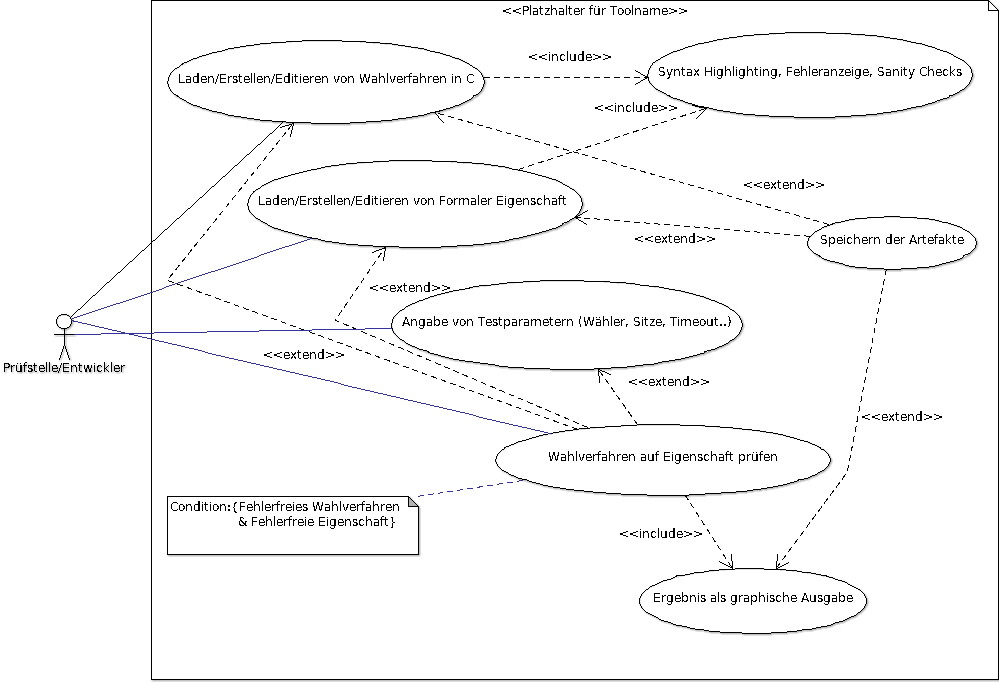
\includegraphics[scale=0.49]{Use-Case-Diagram}}
	
 
\section{Objektmodelle}
\section{Dynamische Modelle}


\chapter{GUI}


\chapter{Phasenverantwortliche}
\section{Pflichtenheft} Justin Hecht
\section{Entwurf} 
\section{Implementierung}
\section{Qualitätssicherung} 
\section{Abschlusspräsentation} 


\chapter{Glossar}
 

 

\listoffigures
 
\end{document}